\chapter[Ferramentas de apoio]{Ferramentas de apoio}

\section{NLTK}

Dado como um conjunto de bibliotecas para processamento de linguagem natural, o NTLK oferece interfaces de processamento para classificação, \textit{"tokenização"}, \textit{“stemming”}, \textit{“tagging”} e análise. Apesar de ser uma biblioteca originalmente norte-americana (e por consequência focada no inglês), os principais módulos do NLTK contam com suporte para o português, como o \textit{stemming} e o módulo de \textit{stopwords}.

O módulo de \textit{stemming} tem como objetivo retirar o sufixo das palavras, de modo que se mantenha apenas o seu radical. Esse método aumenta consideravelmente a chance de palavras sinônimas se corresponderem \cite{marconltk}, melhorando assim a performance geral do analisador de frases. O módulo do \textit{stopwords} também é focado na melhoria da performance, visto que tais palavras agregam pouco valor semântico à frase (mais informações sobre as técnicas citadas na seção \ref{limpeza}). Observe no Listing \ref{lst:nltk} um exemplo de remoção de \textit{stopwords}.

\begin{lstlisting}[language=python, caption=Removendo \textit{stopwords} usando a biblioteca NLTK, label={lst:nltk}]

>>> from nltk.corpus import stopwords 
>>> from nltk.tokenize import word_tokenize 

>>> stop_words = set(stopwords.words('portuguese')) 
>>> example_sent = "Este é um exemplo de frase que podemos remover as palavras vazias"

>>> word_tokens = word_tokenize(example_sent)
>>> filtered_sentence = [w for w in word_tokens if not w in stop_words]

>>> print(filtered_sentence)
['Este', 'é', 'exemplo', 'frase', 'podemos', 'remover', 'palavras', 'vazias', '.']


\end{lstlisting}

\section{scikit-learn}
\label{sec:sklearn}

A biblioteca scikit-learn\footnote{https://scikit-learn.org/stable/} provê algoritmos de aprendizado supervisionado e não-supervisionado através de interfaces pré-definidas. Todos os algoritmos de classificação considerados neste trabalho estão implementados nesta biblioteca.

Além da classificação, o scikit-learn contém outros módulos, como os de regressão e clusterização. Por se tratar de uma biblioteca para mineração e análise de dados, uma série de pacotes é necessária para o seu aproveitamento, como o matplotlib\footnote{https://matplotlib.org/}, o numpy\footnote{https://www.numpy.org/} e o pandas\footnote{https://pandas.pydata.org/}. Esses pacotes fazem parte de uma pacote chamada Pydata. Neste projeto, todos os classificadores utilizados e testados foram providos pelo scikit-learn.

A biblioteca do scikit-learn também possui suporte para a aplicação de técnicas de treinamento e organização do código, como:

\begin{itemize}
    \item \textbf{Pipeline}: uma classe que permite a construção de métodos, compostos por diversos passos e parâmetros variáveis. Nos experimentos realizados neste trabalho, esses passos são as classes responsáveis por extrair os atributos do texto e pelo modelo da classificação.
    \item \textbf{K-fold cross-validation}: uma técnica que visa eliminar o viés gerado ao realizar a divisão do \textit{dataset} entre dado de treino e dado de teste. A técnica propõe solucionar este problema dividindo os dados de treino em \textit{K} partes e realizando o experimento proposto \textit{K} vezes, revezando, em cada iteração, a parte a ser utilizada no teste.

   \item \textbf{GridSearchCV}: uma técnica que realiza uma busca por “força bruta”, para encontrar os hiperparâmetros do modelo de classificação que melhor atendem o problema. Para isso, utilizando o scikit-learn, é definido um conjunto de parâmetros a serem avaliados e o critério de avaliação do método. O GridSearchCV, então, avalia o desempenho do modelo utilizando todas as possíveis combinações dos parâmetros sugeridos. De acordo com a documentação do scikit-learn, a busca pelos parâmetros é otimizada pelo uso da validação cruzada \cite{scikit-learn}.Para um melhor entendimento observe a Figura \ref{kfold} que ilustra o uso do K-fold na etapa de busca de parâmetros.


\begin{figure}[!htb]
    \center{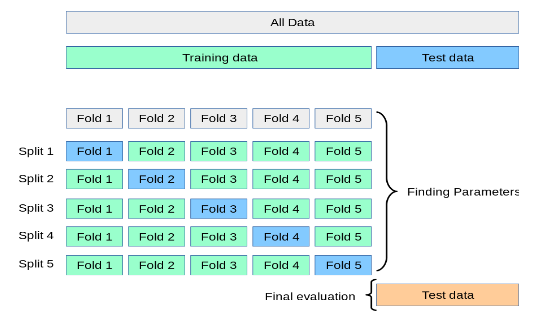
\includegraphics[scale=0.8]
    {figuras/kfold_example.png}}
    \caption{FONTE: scikit-learn.org}
    \label{kfold}
\end{figure}

\end{itemize}

\newpage

\section{Jupyter notebook}

O Jupyter notebook é uma ferramenta que permite não só a execução de código python no navegador, mas também seu gerenciamento, organização e apresentação. Com ela, o desenvolvimento dos algoritmos é facilitado, visto que a execução dos mesmos pode ser separada por “blocos”. Seguindo essa mesma lógica, é possível utilizar-se de comentários em \textit{markdown} para documentar esses blocos de algoritmo, de modo que se facilite tanto a organização, quanto a leitura posterior desses dados. Com todas essas vantagens, o jupyter notebook se tornou nossa principal ferramenta para a realização dos testes. Esta também é uma ferramenta do conjunto Pydata.

\begin{figure}[!htb]
    \label{fig:jupyter}
    \center{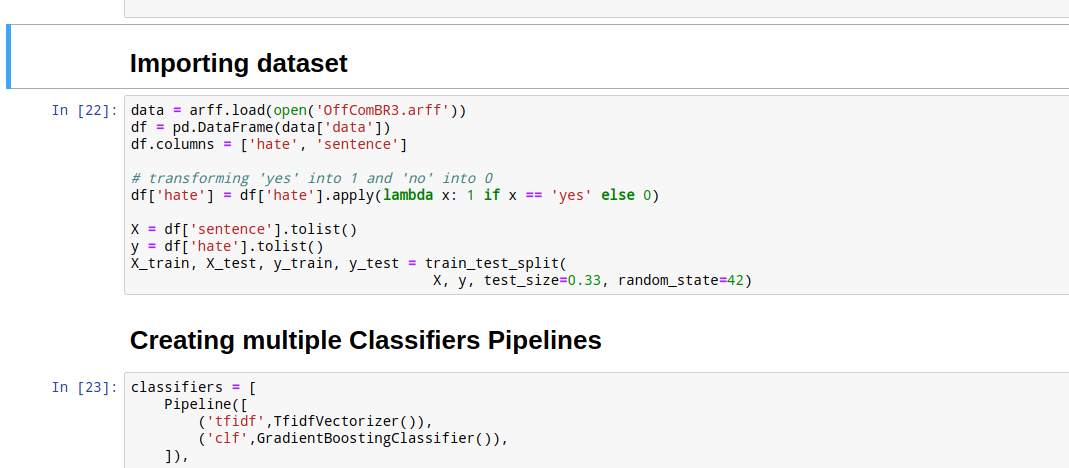
\includegraphics[scale=0.6]
    {figuras/jupyter-note.png}}
    \caption{Screenshot de Jupyter Notebook}
\end{figure}

\section{Conjunto de dados}
\label{sec:dataset}

Um dos desafios enfrentados no atual trabalho foi a busca por um conjunto de dados (\textit{dataset}) categorizado de discurso de ódio que atenda aos requisitos de: ser em português brasileiro, utilizar linguagem coloquial e ser composta por textos pequenos. Estes requisitos foram definidos para que os dados utilizados nos treinos sejam o mais próximo possível do contexto onde o classificador será aplicado.

\begin{center}
\begin{table}[h!]
\centering
\begin{tabular}{ |c|c|c| } 
 \hline
 Tamanho & 1250 frases \\ 
 Discurso de ódio & 419 frases  \\ 
 Média de caracteres. & 72.5  \\
 Média de palavras & 12.8 \\
 \hline
\end{tabular}
\caption{Informações do dataset}
\end{table}
\end{center}

O conjunto de dados encontrado que melhor atende aos requisitos do projeto é o OffComBR \cite{Pelle2017}. A fim de se obter familiaridade com os dados, e como parte da etapa de Entendimento dos Dados do CRISP-DM (mais informações no capítulo \ref{fluxo_atividades}), uma análise exploratória dos dados foi conduzida e algumas informações foram obtidas, como: o \textit{dataset} é composto por mais de mil e duzentos comentários, sendo 419 classificados como discurso de ódio ou conteúdo impróprio. No conteúdo das observações, diferentes assuntos são abordados, como política, economia, futebol e religião. As frases contém uma média de 72 caracteres, porém nenhuma ultrapassa 100 (como é possível observar na Figura \ref{fig:hist-ds}. além de um alto grau de coloquialismo e erros de digitação. Racismo, sexismo, homofobia, xenofobia e intolerância religiosa estão entre os critérios adotados na classificação manual realizada pelos seus colaboradores. Observe, na Tabela \ref{dataset_ex}, as cinco primeiras observações do \textit{dataset}.

\begin{table}[htbp]
\centering
\begin{tabular}{cccccccccc}
\hline
 & \textbf{\begin{tabular}[c]{@{}c@{}}Classe\end{tabular}} & \textbf{\begin{tabular}[c]{@{}c@{}}Frase\end{tabular}} &  \\
 \hline
\textbf{0} & C1 & Votaram no PEZAO agora tomem no CZAO  \\
\textbf{1} & C0 & So conversa mole desde que golpeou o poder nao e Temer  \\
\textbf{2} & C0 & FORA TEMER  ABAIXO A REDEGLOBODECORRUPCAO. \\
\textbf{3} & C1 & VAO BATE PANELASSEUS BURROSBEM FEITO \\
\textbf{4} & C0 & Podiam retirar dos lucros dos bancos
\end{tabular}
\caption{Trechos do dataset escolhido}
\label{dataset_ex}
\end{table}


\begin{figure}[!htb]
    \center{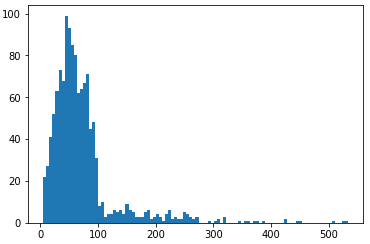
\includegraphics[scale=1]
    {figuras/dataset_info_graphic.png}}
    \caption{\label{fig:hist-ds} No eixo X, quantidade de frases e no eixo Y, quantidade de caracteres}
\end{figure}